\chapter{Ordinary differential equations}

Teaching started on Monday 2019.11.25 (week 48a).

This chapter corresponds to part of chapter 4 in \cite{eck2017mathematical}.

\section{Quantitative analysis of models in population dynamics}

Recall from week 46 (chapter 1) that we had two models for population dynamics.

\begin{itemize}
  \item The first one, the exponential model was described by
    \[
      x'(t) = px(t),\quad p \in \R,
    \]
    where $p$ was the growth rate.
  \item The second, the constrained model was described by
    \[
      x'(t) = qx_M x(t) - q x^2(t),\quad q, x_M \in \R
    \]
    where $q > 0$ was the growth rate and $x_M$ was the maximum carrying
    capacity of the environment in number of individuals.
\end{itemize}

Both of these models share the common mathematical structure of an autonomous
equation, i.e. an equation of the form
\begin{align}
  \label{eq:autonomous-ode}
  x'(t) = f(x(t)),
\end{align}

where $f$ (read $x'$) does not depend explicitly\footnote{That is, $f$ cannot
\textit{unwrap} $t$ out of $x(t)$ and do anything with it alone, it has to work
on $x(t)$ as its variable.} on $t$.

In this section we will focus on the qualitative aspects of the model, i.e.
what information can we get from it without explicitly solving the equations
(which in this case we can, but in the next examples we won't).

Recall that a \textbf{stationary solution} of an ODE is one that stays constant
in time, i.e. of the form $x(t) = c$. How can we find them? Easy, if $x$ is
constant then we must have $x'(t) = f(x(t)) = 0$. For our previous models this means
\begin{itemize}
  \item $x(t) = 0$ for the exponential model, and
  \item $x(t) = 0$ or $x(t) = x_M$ for the second model. We get these two
    solutions from solving
    \[
      x'(t) = qx_M x(t) - qx^(t) = 0
    \]
    for $x(t)$ using the well known quadratic formula.
\end{itemize}

We are interested in these solutions because they are predictable and
\textit{don't blow up} as time passes. Later in this chapter we will formally
define the concept of stability and quantify how stable solutions are based on
how close they are to the stationary solutions.

\subsection{Introduction to linear stability analysis}

For now we will settle with something called \textbf{linear stability
analysis}. The main idea is to linearise the solution (i.e. Taylor expand up to
degree 1) a stationary solution. Let $x^*$ be a stationary solution to an
autonomous problem of the form \ref{eq:autonomous-ode}. The linear expansion we are talking about is
\[
  f(x) = f(x^*) + f'(x^*)(x - x^*) + O(\abs{x - x^*}).
\]
To make things easier, let us take $y(t) = x(t) - x^*(t)$. We shall ignore the
error term $O(\abs{x - x^*}) = O(y(t))$ and thus we get
\begin{align}
  \label{eq:stationary-linear-exp}
  y'(t) = f'(x^*) y(t).  
\end{align}
Now, \ref{eq:stationary-linear-exp} is trivial to solve explicitly---it is a
linear homogeneous equation with constant coefficients
\[
  y(t) = c e^{f'(x^*) t}.
\]
Intuitively, as $t \to \infty$ we have
\[
  \abs{y(t)} \to 0  \implies \abs{x(t) - x^*(t)} \to 0 \iff x(t) \to x^*(t),
\]
i.e. the linearised solution $y(t)$ converges to the stationary solution
$x^*(t)$.

More on this later.

\section{Predator--prey models}

\subsection{Derivation of the Lotka--Volterra equations}

Now we turn our attention to environments where there are two species and one
eats/hunts/harvests the other. Let us model this from scratch to get yet
another example of how things work in Mathematical modelling. For this
derivation we shall use the following assumptions.

\begin{enumerate}
  \item The prey population has unlimited resources available for its growth all the time.
  \item The predator population feeds exclusively on the prey population.
  \item TODO: Something i cant remember.
  \item The rate of growth of the populations is proportional to their size.
  \item The environment is stable over time.
\end{enumerate}


We now proceed with the standard recipe for deriving models.

\begin{enumerate}
  \item \textbf{Name the quantities involved in the problem.} We are trying to
    model how two populations change over time so we need
    \begin{align*}
      \begin{array}
        {cl}
        t &:= \text{ time} \\
        x_1(t) &:= \text{ size of prey population at time } t \\
        x_2(t) &:= \text{ size of predator population at time } t
      \end{array}
    \end{align*}

  \item \textbf{Find relations between the quantities.} From assumption X we
    now that the growth of both species is directly proportional to the size of
    the populations, in other words
    \[
      x_1' = p_1 x_1\text{ and } x_2' = p_2 x_2.
    \]
    A priori, we don't know if $p_1$ depends only on $t$ or on $x_2(t)$ or on
    both. The possibility that $p_1$ depends on $x_1(t)$ is ruled out by the
    assumption that growth is proportional to size. Looking at the assumptions
    once more we find that $p_1$ cannot depend on $t$ since ``the environment
    is stable over time''. There fore it must be that $p_1$ is a function only
    of $x_2(t)$, which really makes sense, since the size of the prey species
    depends on how many individuals are being eaten by the predator species. A
    similar argument for $p_2$ yields
    \[
      p_1(x_2(t))\text{ and } p_2(x_1(t)).
    \]
    
    But what do these functions $p_1$ and $p_2$ look like? Well, the prey
    population naturally grows since we assumed unlimited resources but at the
    same time it is being eaten at some rate by the predator population.
    Similarly, the predator population naturally dies unless they can feed on
    the prey population. We introduce the parameters $\alpha, \beta, \gamma,
    \delta > 0$ and formalise these relations with
    \begin{align*}
      p_1(x_2(t)) = - \beta x_2(t) + \alpha 
      \qquad \text{ and } \qquad
      p_2(x_1(t)) = \delta x_1(t) - \gamma.
    \end{align*}

    Finally we get our model, commonly referred to as the Lotka--Volterra
    equations, derived independently by both authors from around 1920 to around
    1925 \cite{lotka-volterra}.
   
    \begin{align}
      \label{eq:lotka-volterra}
      \begin{cases}
        x_1' &= (\alpha - \beta x_2) x_1 \\
        x_2' &= (\delta x_1 - \gamma) x_2
      \end{cases}
      .
    \end{align}
\end{enumerate}

The mathematical structure of this problem is that of an planar
system of autonomous ODEs. We may rewrite it as
\begin{align}
  \label{eq:autonomous-planar-sys}
  \begin{cases}
    \vec{x}'     &= f(\vec{x}) \\
    \vec{x}(t_0) &= \vec{x_0}
  \end{cases}
\end{align}
with $f : \Omega \subseteq \R^2 \to \R^2$. If $f$ is sufficiently nice (i.e.
locally Lipschitz) then an initial value problem of the form in
\ref{eq:autonomous-planar-sys} has locally unique solutions. However, it is not
the explicit solutions that interest us right now, but rather the qualitative
aspects of their behaviour.

\subsection{Qualitative analysis of the Lotka--Volterra equations}

We look into the stationary solutions to later look at stability. Once more,
setting $x_1, x_2 = 0$ in \ref{eq:lotka-volterra} gives us the stationary
solutions

\begin{align*}
  \left(
    \begin{array}
      {c}
      x_1 \\ x_2
    \end{array}
  \right) = \left(
    \begin{array}
      {c}
      0 \\ 0
    \end{array}
  \right) \qquad \text{ and } \qquad \left(
    \begin{array}
      {c}
      x_1 \\ x_2
    \end{array}
  \right) = \left(
    \begin{array}
      {c}
      \alpha / \beta \\ \gamma / \delta
    \end{array}
  \right).
\end{align*}

There are too many parameters to work comfortably with this solutions. Let us
non-dimensionalise before moving on to get rid of as many parameters as we can.
Very quickly, we choose the fundamental dimensions $T$ for time and $N$ for
number of individuals and carry out a dimensional analysis to get
\[
\begin{array}{rlcrl}
  [t]                   & = T                                   & \qquad & [x_1] = [x_2]                                & = N \\
  \left[ \alpha \right] & = \left[ \gamma \right] = \frac{1}{T} &        & \left[ \beta \right] = \left[ \delta \right] & = \frac{1}{NT}
\end{array}
.
\]
We choose the characteristic quantities $\overline{x_1}, \overline{x_2}$ and
$\overline{t}$ and set up the change of variables
\[
  z_1 = \frac{x_1}{\overline{x_1}},\qquad
  z_2 = \frac{x_2}{\overline{x_2}} \qquad \text{ and } \qquad
  \tau = \frac{t}{\overline{t}}.
\]

Substitute with care in \ref{eq:lotka-volterra} (careful with the derivatives) to get
\[
  \begin{cases}
    z_1' &= \overline{t} \alpha z_1 - \beta \overline{x_2} \overline{t} z_1 z_2 \\
    z_2' &= \delta \overline{x_1}\overline{t} z_1 z_2 - \gamma \overline{t} z_2
  \end{cases}.
\]
Notice how we have four different coefficients for $z_1$ and $z_2$ but only
have three characteristic quantities. This means we'll need to make a
compromise. Which one to make is dictated by our taste and the mathematical or
biological interpretation of the parameters we choose. We will not do all four
options here but the Lotka--Volterra equations often come with
\[
  \overline{t} \alpha = 1,
  \qquad \beta \overline{x_2} \overline{t} = 1 \qquad \text{ and } \qquad
  \delta \overline{x_1} \overline{t} = \gamma \overline{t},
\]
which in turn give us the \textbf{non-dimensionalised version of the
Lotka--Volterra equations}
\begin{align}
  \label{eq:non-dim-lotka-volterra}
  \begin{cases}
    z_1' &= (1 - z_2) z_1 \\
    z_2' &= a (z_1 - 1) z_2
  \end{cases},
\end{align}
where there is only one parameter $a = \gamma / \alpha$. 

In this form, the stationary solutions are given by
\[
  \vec{z} = \left(\begin{array}{c}0 \\ 0\end{array}\right),
  \qquad \text{ and }\qquad
  \vec{z} = \left(\begin{array}{c}1 \\ 1\end{array}\right).
\]


\subsubsection{Directional field of the Lotka-Volterra equations}

Plotting the directional field is a tool that proves useful when we want to get
an overall idea of how the system behaves. Recall that given an autonomous ODE
of the form $\vec{x}' = f(\vec{x})$ the directional field is a vector field of
the form $x \mapsto f(x)$. In two dimensions this corresponds to a graph where
the axes represent the values that the functions $x_1$ and $x_2$ can take and
the arrows point in the direction $(f_1(x), f_2(x))$.

It is hard to draw these diagrams by hand but there are a number of steps we
can take to get an idea of what they look like. Let's go back to the
Lotka-Volterra model in the non-dimensionalised form. We plot the directional
field by following these steps

\begin{enumerate}
  \item \textbf{Find the stationery solutions.} These become points in the vector field
    since $f(x) = 0$ by definition of stationary solution (and therefore there
    is no arrow to draw).
  \item \textbf{Find the isoclines}, i.e. the curves\footnote{Here we mean
    \textit{curve} in the most general sense---isoclines can be straight lines
  or curves and they can be disjoint as is the case in this example.}
    \begin{align*}
      N_1 &= \{f_1 = 0 \} = \{\vec{z} \mid f_1(\vec{z}) = 0\} = \{(z_1, z_2) \mid f_1(z_1,z_2) = 0\} \\
      N_2 &= \{f_2 = 0 \} = \{\vec{z} \mid f_2(\vec{z}) = 0\} = \{(z_1, z_2) \mid f_2(z_1,z_2) = 0\}
    \end{align*}
  \item \textbf{Find the areas of monotonicity}, i.e. the regions of the plane given
    by\footnote{It is useful to write them as an intersection since therefore
      we can reuse the sets $\{f_n < 0\}$ and $\{f_n > 0\}$ to calculate all
    the regions depending on how they overlap.}
    \begin{align*}
      D_{++} = \{f_1 > 0\} \cap \{f_2 > 0\} \\
      D_{+-} = \{f_1 > 0\} \cap \{f_2 < 0\} \\
      D_{-+} = \{f_1 < 0\} \cap \{f_2 > 0\} \\
      D_{--} = \{f_1 < 0\} \cap \{f_2 < 0\} \\
    \end{align*}
    Keep in mind that the isoclines tell us where there is a change from one
    area of monotonicity to another\footnote{The reason for this is that we
      normally ask that the functions involved in the ODE are \textit{nice
      enough}, i.e. at least $C^2$ which means that the derivatives are
    continuous.}.
  \item \textbf{Draw the vector field}, i.e. some arrows.
\end{enumerate}

\begin{figure}
  [h]
  \centering
  \incfig[0.8]{lotka-volterra-direction-field-handmade}

  \caption{Sketch of the direction field for the Lotka-Volterra equations.}
\end{figure}

\begin{figure}
  [h]
  \centering
  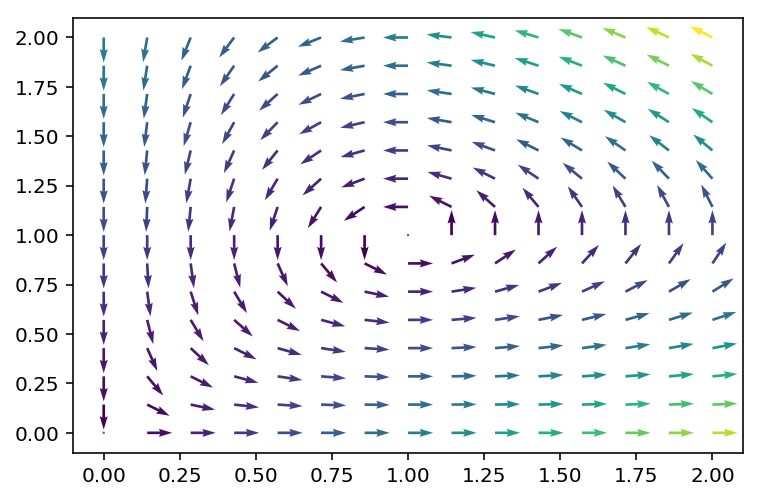
\includegraphics[width=0.8\columnwidth]{figures/lotka-volterra-direction-field.png}

  \caption{Direction field for the Lotka-Volterra model with $a = 0.5$ generated by a computer.}
\end{figure}

In the computer generated picture it is probably easier to tell what is
happening with the solutions. If one were to choose a point in the plane, a
solution going through that point would move in the direction of the vector in
that point. Repeating this process can give us a rough idea of what the
solutions look like: orbits around the stationary solution $(1,\ 1)$.


\subsection{Phase diagram of the Lotka-Volterra equations}

In our qualitative analysis of the Lotka-Volterra model we have found the
stationary solutions and more or less characterised the rest of the solutions
using the direction field. We would, however, like to have a more precise idea
of what the solutions look like. We will devote the rest of this section to
that.

\begin{dfn}
  [First integral]

  TODO. we really need a definition here :(
\end{dfn}


\section{Stability theory}

Consider the general autonomous system
\begin{align}
  \label{eq:autonomous-stability}
  \vec{x}' = f(\vec{x})
\end{align}
where $f: \Omega \subset \R^n \to \R^n,\ \Omega$ is open and $f \in
C^2(\Omega)$.

\begin{dfn}
  [Lyapunov stability] Let $\vec{x}^*$ be a stationary solution to
  \ref{eq:autonomous-stability}. We say $\vec{x}^*$ is Lyapunov stable (or just
  stable for short) if for every open neighbourhood $U$ of $\vec{x}^*$ there
  exists an open neighbourhood $V$ of $\vec{x}^*$ such that any solution
  $\vec{x}$ of \ref{eq:autonomous-stability} with $\vec{x}(0) \in B$ satisfies
  $\vec{x}(t) \in U$ for all $t > 0$.
\end{dfn}

\begin{dfn}
  [Asymptotic stability]

  Let $\vec{x}^*$ be a stationary solution to \ref{eq:autonomous-stability}. We
  say $\vec{x}^*$ is asymptotically stable if there exists an open
  neighbourhood $W$ of $\vec{x}^*$ such that for any solution $\vec{x}$ of
  \ref{eq:autonomous-stability} with $\vec{x}(0) \in W$ it holds that
  \[
    \norm{\vec{x}(t) - \vec{x}^*} \to 0 \text{ as } t \to \infty.
  \]
\end{dfn}

\begin{remark}
  If $\vec{x}^*$ is asymptotically stable then it is Lyapunov stable.
\end{remark}

\subsection{Linear stability analysis}

\begin{dfn}
  Let $\vec{x}^*$ be a stationary solution to \ref{eq:autonomous-stability}.
  The linear system
  \begin{align}
    \label{eq:linear-system-stability}
    \vec{y}' = Df(\vec{x}^*)\vec{y}
  \end{align}
  is called a linearisation of \ref{eq:autonomous-stability} in $\vec{x}^*$.

  Moreover, $\vec{x}^*$ is called linearly unstable, resp. stable /
  asymptotically stable if $\vec{0}$ is unstable, resp. stable / asymptotically
  stable for \label{eq:linear-system-stability}.
\end{dfn}

\begin{thm}
  [Principle of linearised stability]

  If $\vec{x}^*$ is linearly asymptotically stable, resp. unstable, then
  $\vec{x}^*$ is asymptotically stable, resp. unstable.
\end{thm}

\begin{remark}
  The previous theorem does not work for Lyapunov stability, i.e.
  \[
    \vec{x}^* \text{ linearly stable } \nRightarrow \vec{x}* \text{ stable}.
  \]
\end{remark}


